\section{Sunday 0603}

\subsection{Morning Keynote: The moment when the future fell asleep}
Professor Kevin Knight
\paragraph{Decipher}
Deciphering of some ancient languages.\\
Decipherment is the original NLP problem.

\paragraph{Generative model for cipher}
\begin{figure}
	\centering 
	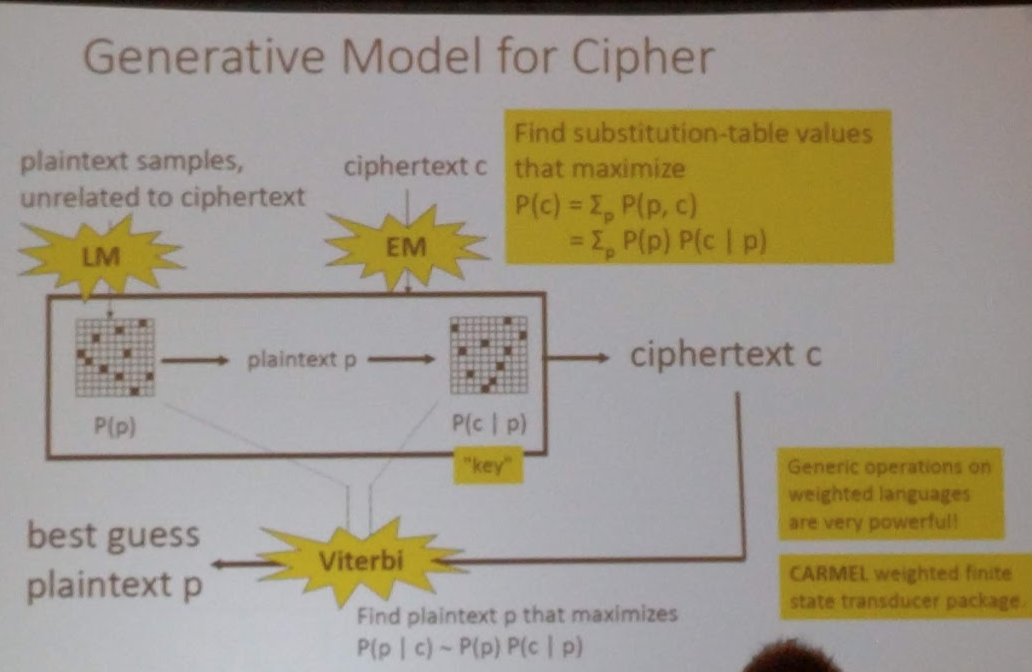
\includegraphics[scale=0.8]{fig0603/kn-cipher-model}
\end{figure}

\paragraph{Recent works}
\begin{itemize}
\item Pixel image -> OCR + decipher in the system -> plain text. No supervision segment and clustering. After that, apply noisy-channel methods with plaintext language model.
\item Zodiac cihpers: Z340, Z32, Z13
\item Improve on the plaintext language models might lead to lower decipher error.
\end{itemize}

\paragraph{Poetry generation}
\begin{itemize}
	\item Can generate poets e.g.: Ghazycininejad, Shi, Choi, Knight EMNLP 2016
	\item Hafez: an interactive poetry generation system (Ghazvininejad et al. ACL demo 2017)
\end{itemize}
\begin{figure}[h]
	\centering 
	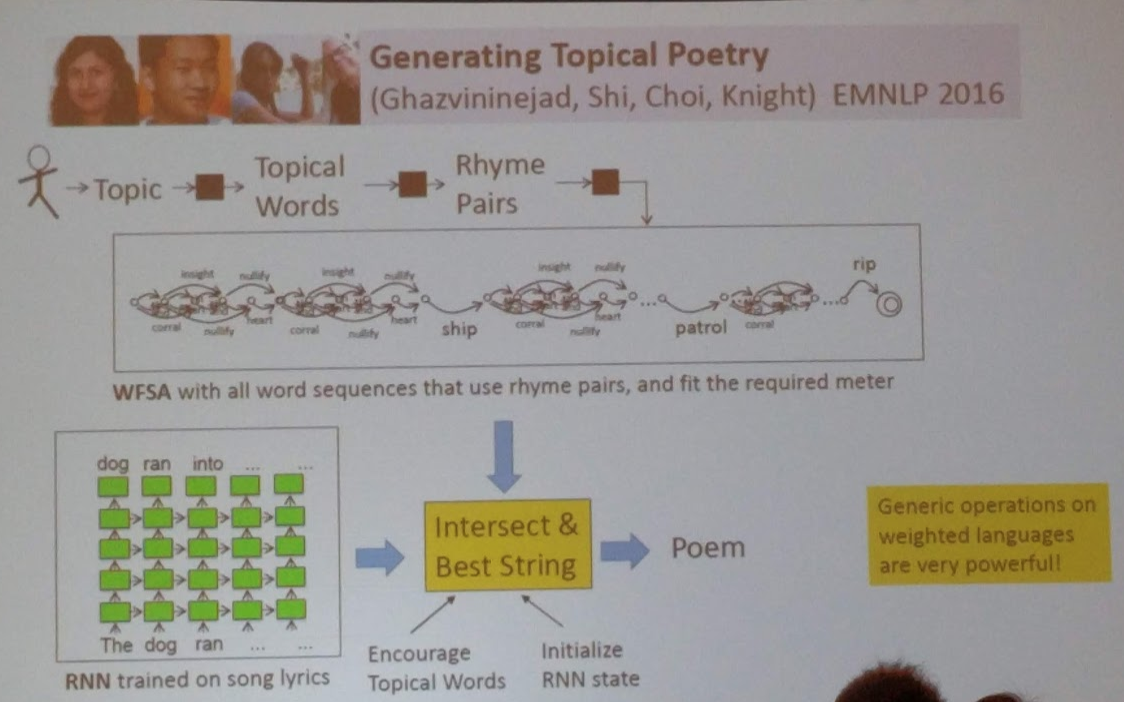
\includegraphics[scale=0.8]{fig0603/kn-generate-poetry}
\end{figure}

\paragraph{RNNs for storytelling}
\begin{itemize}
	\item How to memorize a random 60-bit string?
	\item RNNs as weighted language recognizers \cite{Chen2018Recurrent}
	\item Does string-based NMT learn source syntax? (EMNLP 2016)
	\item Why neural translations are the right length? (EMNLP 2016). 
	\item Towards controllable story generation? (Peng et al., NAACL 2018 storytelling workshop) 
	\item Paper anstract writing through abstract mechanism (Want et al, ACL 2018)
	\item Neural poetry translation \cite{Ghazvininejad2018Neural}
\end{itemize}

Why do automatic outputs look so different (to us) than what was trained on?

\paragraph{Conclusions}
Still a long way to go. NLP for entertainment, commerce.


\subsection{Morning Posters}

\subsubsection{FEVER: a large scale dataset for fact extraction and verification \cite{Thorne2018FEVER:}}
\begin{itemize}
	\item A dataset containing 185,000 facts. Each wiki passage (?) has (humanly labeled) several claims (true or false).
\end{itemize}

\subsubsection{Efficient sequence learning with group recurrent networks \cite{Gao2018Efficient}}
\begin{itemize}
	\item Sequence learning task.
	\item Divide the hidden layer into two parts, so that computation is more efficient.
	\item Mix two parts of the hidden representation by the rearrange() function, so that the inter-group correlation can be considered more.
\end{itemize}

\subsubsection{Embedding syntax and semantics of prepositions via tensor decomposition \cite{Gong2018Embedding}}
\begin{itemize}
	\item Train a word embedding considering the tensor decomposition and preposition embeddings.
	\item The loss function contains ALS model term and the bias scalar parameters.
\end{itemize}

\subsubsection{Semi-supervised event extraction with paraphrase clusters \cite{Ferguson2018Semi-Supervised}}
\begin{itemize}
	\item First cluster the articles. Then identify "easy" events (after running a pre-trained supervised system on all sentences). Select most likely triggers for "hard" mentions.
\end{itemize}




\subsection{Machine Learning 3}
Empire A
\subsubsection{Deep generative model for joint alignment and word representation \cite{Rios2018Deep}}
\begin{itemize}
	\item Optimize the variational lower bound of the marginal likelihood of a sentence pair: $P_\theta (x_i^m, y_j^n | m, n)$ where $x_i^m$ and $y_j^n$ are word observations in languages 1 and 2 respectively.
\end{itemize}


\subsubsection{Evaluating the stability of embedding-based word similarities}
\begin{itemize}
	\item Cosine similarities are not satable. They have biases w.r.t corpus from which the word2vec are trained.
	\item Question: what do embeddings represent? They measure the properties of a curated corpus, not the word themselves.
	\item Two views of embeddings: downstream-centered or corpus-centered. (This work focus on the corpus-centered view)
	\item The embeddings are calculated using LSA (latent semantic analysis + tf-idf using \texttt{sklearn}), SGNS (skip-gram with negative sampling), GloVe, and PPMI (positive point-wise mutual information). Each methods contain fixed, shuffled, and bootstrap settings.
	\item Measure the cosine similarity bound of 20 query words. Those with lower variances is more stable.
\end{itemize}

\takeaway{Should study from the methodology for designing experiments.}

\subsubsection{Learning word embeddings for low-resource language PU learning \cite{Jiang2018Learning}}
\begin{itemize}
	\item Problem: large datasets are required to train datasets. Might be hard to find this large of corpus for low-resource languages. (this project focus on those with low-resource, but not those very-low-resource languages)
	\item Problem: Sparsity of the co-occurrence matrix (>99\% of them are zero). Can be true zeros or missing entries (can co-occur but just has not in the given corpus)
	\item Motivation: word2vec use negative sampling, which only subsamples for some of the not mentioned.
	\item Propose a PU-learning framework for training word embedding. The learning alg deals wiht all negative pairs.
	\item Three components in the framework: 
	(1) Pre-processing (building the o-occurrence matrix -> scale counts by PPMI metric w.r.t [Levy '15]) 
	
	(2) PU-learning for matrix actorization: $A \approx W^T H$, where we try to optimize (using coordinate descent)
	(see paper for the equations)
	
	(3) Post-proessing. Average $w_i^T$ and $h_i$ to get the resulting word vector.
\end{itemize}


\subsection{Afternoon keynote: building innovative startups, products, and services -- personal insights}
Daniel Marcu (Amazon)
\begin{itemize}
	\item Hard to annotate all domains -- they are just too many of them. Very important therefore to enable domain adaptation.
	\item Commercial requirements usually forces us to be short-sighted.
	\item The most important lesson: We owe success to those people we worked with.
	\item Example of exploration in NMT structures.
	\item Important to know that the world is not just the pinnacle we focus on (e.g., in PhD). The world is the whole circle (big picture) -- much more than what you have been focusing on pushing.
	\item Q: expectation between tech people and marketing people. People might like to go hype; also scientists should not make overly promising claims.
	\item Some tasks are hard to evaluate. These will be what a lot of future projects work on. e.g: quality of Alexa communication.
\end{itemize}

\subsection{Afternoon Posters}
\subsubsection{Diverse few-shot text classification with multiple metrics \cite{Yu2018Diverse}}
\begin{itemize}
	\item Task: Few-shot learning in diverse tasks.
	\item Propose an adaptive metric learning approach that automatically determines the best weighted combination from a set of metrics obtained from meta-training tasks for a (new) few-shot task.
	\item Matrix-completion based task clustering
\end{itemize}

\subsubsection{Cross-lingual learning-to-rank with shared representations \cite{Sasaki2018Cross-Lingual}}
\begin{itemize}
	\item Task: For each query-document pair, learn a mapping. More specifically, a query CNN and a document CNN compress the query and document into a hidden embedding.
	\item Several models to learn transferrable knowledge between languages. A basic "cosine model" minimizes the cosine similarity between the query and document embeddings. This does not work well on low-resource languages.
	\item A deep model adds a MLP to learn a similarity score given the embedding. How to make this model work on low-resource setting?
	\item Parameter-sharing is the improvement. Use the query CNN and the MLP trained on a high-resource language, and fine-tune using a low-resource language.
\end{itemize}


\subsubsection{Are all languages equally hard to language-model? \cite{Cotterell2018Are}}
\begin{itemize}
	\item Hypothesis: inflectional morphology makes a language hard to model. LM performance negatively correlated with morphological counting complexity.
	\item Correlation disappears when modeling lemmata instead of forms.
	\item Different languages contain varying bits per (English) character.
	\item The comparison methods are the takeaways at the end of the day.
\end{itemize}


\subsection{Text Mining 1}
\subsubsection{Explainable prediction of medical codes from clinical text}
\begin{itemize}
	\item Task: the clinical coding problem
	\item Model: word embed -> CNN features -> attend (one for each label) -> classifier (Logistic Regression)
\end{itemize}

\subsubsection{Event-time extraction with a decision tree of neural classifiers \cite{reimers2018event}}
\begin{itemize}
	\item Temporal links annotations
	\item Problem: sparse annotation of event times.
	\item TLINK annotation: dense annotation of event times. (ACL '16)
	\item Temporal anchoring of events given complete documents.
	\item Dataset: TimeBank-EventTime Corpus
\end{itemize}

\subsection{Test of Time}
Empire B

\subsubsection{Remembrance of Aravind Joshi}
\begin{itemize}
	\item 1929 - 2017
	\item Centering: a framework for modeling the local coherence of discourse; the penn discourse treebank; tree adjoining grammars.
\end{itemize}

\subsubsection{BLEU}
\begin{itemize}
	\item ACL 2002, Kishore et al.
	\item "Bilingual Evaluation Understudy": compare short runs of candidate text against reference translations.
	\item Not necessary to match pair-wise
	\item All words are equally important: all you need is a tokenizer. Set up a brevity penalty BP:
	\[BP=\left\{ \begin{matrix} 1 \text{if c > r}  \\ e^{1-r/c} \text{otherwise} \end{matrix}  \right. \]
	\item Modified u-gram precision: average log with unit weights.
	\item BLUE = $BP \times exp(\sum_n w_n log p_n)$  where $p_n$ is the n-gram precision, and positive weights $w_n$ sum up to 1.
	\item Stunningly simple, surprisingly simple.
\end{itemize}

\paragraph{Retrospective}
\begin{itemize}
	\item Context: DARPA: slow and expensive for human evaluations; long pause in funding.
	\item Hard to sell in 2002: "quantity leads to quality". "Don't attempt to divine human judgment for every sentence. Rather, average out individual sentence judgment errors over a corpus."
	\item Polarization: people have polarized reviews towards BLEU.
	\item It is an understudy -- never meant to replace human judgments.
	\item Q: criticism that BLEU penalizes stylicism? A: wow the metrics actually understand language.
\end{itemize}

\subsubsection{Structured Perceptron}
\begin{itemize}
	\item EMNLP 2002, "Discriminative Training Methods for HMM", Michael Collins
	\item Background: structured prediction problems
	\item Dominant approach in the 1990s to do structured prediction as density estimation: model $p(x, y)$ or $p(y|x)$. e/g: Log-linear history-based models.
	\item Method: POS Tagging with HMMs
	\item Generalization bounds. (written in a PAC-style).
	\item Conclude: thoughts about learning and search.
	
	Approach 1: global training. e.g: CRF log-loss, max-margin
	
	Approach 2: Local training, etc., seq2seq
	
	\item Some hypotheses in 2002: (1) search is necessary for some structured prediction problems. (2) If you believe search is beneficial, then local normalization does not work. (3) Generalization bounds will be important in a scientific understanding of why / how machines learn. (see Dziugaite and Roy on PAC-Bayes for NN)
	
	Interesting to think about them.
\end{itemize}

\subsubsection{A sentiment Odyssey}
\begin{itemize}
	\item EMNLP 2002, Thumbs up? Sentiment classification using ML techniques by Bo Pang et al.
	\item Background: people start to use internet increasingly prevalently. Then sentiment analysis is increasingly important. Also the dataset sizes were pretty small.
	\item Released the imdb movie review dataset.
	\item Inspirational slide? Do something interesting but that might not be deemed interesting as considered by other people. Since most people here have done PhD they should know how to get out of it. 
\end{itemize}


